%!TEX root = ../report.tex

\begin{document}
    \chapter{State of the Art}
	\label{chap:stateofart}
	Introduction to the modern deep learning and their impact onto the various vision tasks are described in the \nameref{sec:deeplearn} section. Information fusion in the temporal domain to fuse information is explained in \nameref{sec:tempfuse}. State of the art segmentation of the input images, in particular semantic segmentation task is illustrated in the \nameref{sec:semseg} section. State of the art segmentation in the classical era and in modern deep learning play crucial role in the temporally fused semantic segmentation. However, there is very little work of fusing the camera pose onto the segmentation task in temporal fashion. More details are discussed in the \nameref{sec:semseg}. Finally chapter \ref{chap:stateofart} is ended with the discussion on the limitations of the previous work with respect to the temporal fusion. 
	
    \section{Deep Learning}
    \label{sec:deeplearn}
    
    Deep learning is a sub field of machine learning that aims to learn the features present in the data by utilizing the hierarchical architectures. The area deep learning falls in the artificial intelligence is depicted in the picture \ref{fig:DLAI}
    
    \begin{figure}[h]
    	\centering
    	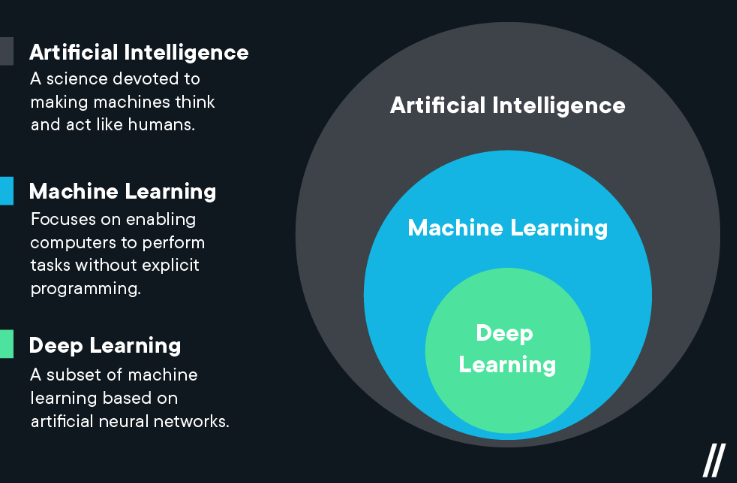
\includegraphics[width=10cm]{images/mldl.png}
    	\caption{Deep learning in the artificial intelligence domain. Courtesy of \cite{35_mldl}}
    	\label{fig:DLAI}
    \end{figure}  
    
    Classical machine learning system uses the raw input and domain expert carefully represent the data as a feature vector from which the data is fed to the models to learn the patterns and classify into appropriate classes \cite{36_lecun2015deep}. 
    Deep learning is a representation learning that takes raw data and find the patterns in the data with different levels of representation in the multiple layers \cite{36_lecun2015deep}. Deep learning can learn any complex representation of the data. For example, a image is represented as pixels and are fed to the neural network, at each layer of the network different feature are learned. In the first layer, higher level features such as edges at a specific orientation and location is determined. In the second layer motifs are learned and so on. The important aspect of the deep learning is that the features are not designed by the field expert rather than learned from the data with a specific set of learning procedures \cite{36_lecun2015deep}.
    
    Many current state of the art learning models uses the deep learning approach to learn the complex function from data. Currently deep learning method can be found in image recognition \cite{37_farabet2012learning}, speech technologies \cite{38_hinton2012deep}, discovery of drug molecule \cite{39_patel2020machine} , understanding the particle accelerator data \cite{40_ciodaro2012online}, DNA sequencing \cite{41_zhang2021deep}, ,and natural language processing \cite{42_hirschberg2015advances}. 
    
    Computer vision is the field of computer science that deals with replicating the functionalities of the human visual system. Traditionally computer vision solved the vision problem by finding the hand crafted features. However, the performance of the classical apporach is outperformed by the advancement of the deep learning based methods. Hand crafted feature descriptors such as Speeded Up Robust Features (SURF),  Hough Transforms are used as feature vectors for the classical machine learning methods for learning \cite{46_o2019deep}. Deep learning methods automatically learns the patterns from the data. Computer vision solves wide variety of problems in the perception domain. Latest approaches helps to solve the detection \cite{44_mohanty2016using}, \cite{45_han2021ecological}, classification \cite{43_srivastava2021comparative}, image synthesis and segmentation tasks \cite{47_minaee2021image}.
    
    Temporal data are the time varying information and can be commonly observed in financial portfolio management, accounting, medical records, inventory management, data from airline, hotel, train industries contains time component with it \cite{48_jensen1999temporal}. Video data are constructed from combining time variant frames and is a common example of a temporal data. Temporal fusion deals with combining of the past information into the current step computation with a aim of improved performance. 
    
    In general approach segmentation is done frame by frame or by skipping in between frames and computing the segmentation on the nth frame. Temporal fusion can be applied in these settings to perform improved segmentation task by combining the past rich information in the current step. 
     
    \section{Temporal Fusion}
    \label{sec:tempfuse}
    
	Temporal fusion can be defined as the process of fusing the temporal data onto the current step with a aim of improving the performance of the model. Temporal data can be observed in many fields such as social media, healthcare, accounting, agriculture, transportation, physics, crime data, traffic dynamics and climate science \cite{49_atluri2018spatio}. Temporal data can be encountered with different data types, Common data types are video, audio, tabular data, and sensors data. Forecasting is a common application of temporal fusion. Multi horizon forecasting is a important problem in the domain of time series. Multi horizon forecast allow the user to optimize the process across the entire path. A novel Temporal fusion Transformer (TFT) \cite{50_lim2021temporal} is a attention based DNN architecture for forecasting by fusing the important past features into the current step. Temporal fusion play a major role in the improved video action recognition. Temporal fusion helps in two ways, firstly by understanding the temporal data the accuracy of the recognition for the dynamic action is improved, secondly removing the redundant temporal data saves the computation overhead. A temporal fusion network known as the AdaFuse, fuses the current and past features with a goal of improved accuracy and efficiency \cite{51_meng2021adafuse}. A temporal non parametric fusion aims to fuse the 
	temporal pose data to the computation of the depth map thereby improving accuracy and efficiency \cite{52_hou2019multi}. The architecture of the multi view stereo can be depicted in the Fig \ref{fig:mvs}. An online multi view depth prediction approach where the depth estimated in the previous step is fused onto the current step in a sensible manner. The network is named as DeepVideoMVS and it is based on the encoder decoder architecture. A ConvLSTM is placed at the latent space to fuse the information from the previous step. The proposed approach outperformed all the existing state of the art multi view stereo method evaluated on the standard metrics \cite{53_duzceker2021deepvideomvs}. 
	A Multiple Fusion Adaptation (MFA) method improves the segmentation accuracy on a unlabeled datasets. Three fusion approach was proposed under MFA, cross model fusion, temporal fusion and novel online-offline pseudo labels. The MFA produced improved semantic segmentation result of 58.2\% and 62.5\% on GTA5-to-Cityscapes and SYNTHIA-to-Cityscapes respectively \cite{54_zhang2021multiple}.  
    
    \begin{figure}
    	\centering
    	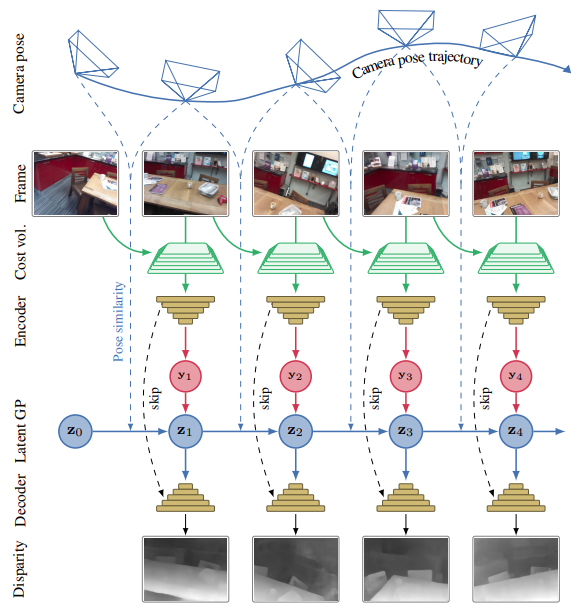
\includegraphics[width=6cm]{images/MVS.png}
    	\caption{Mulit view stereo architecture for depth estimation. Courtesy of \cite{52_hou2019multi}}
    	\label{fig:mvs}
    \end{figure} 	

    \section{Semantic Segmentation}
    \label{sec:semseg}
    
    Humans can perceive the surrounding environment and make sense of it with high accuracy. Due to the advancement of computer vision these capabilities are transferred to the machines, performing even better than humans. Today, we have computer vision models that can detect objects, find shapes, track the object movement and perform action based on the data. Computer vision is most commonly used in the autonomous driving cars, aerial mapping, surveillance applications, virtual reality and augmented reality and so on. One of the common problem in computer vision is labeling the each pixels of the image to a particular categories. Also known as the segmentation. Mathematically image segmentation can be defined as
     
    If $I$ is set of all image pixels of a image, then segmentation generate unique regions ${S_1, S_2, S_3, S_4,....S_n}$ such that combining all these regions will return $I$. 
   
    Image segmentation can be classified into three categories Semantic segmentation, Instance segmentation and Panoptic segmentation. Semantic segmentation finds the shape, size and form of the objects in addition to their location. Instance segmentation finds one more parameter of number of unique object present in the image. Panoptic segmentation is the combination of the semantic and instance segmentation. The difference between all the types of semantic segmentation can be observed in the Fig \ref{fig:SS}.
    
    \begin{figure}[h]
    	\centering
    	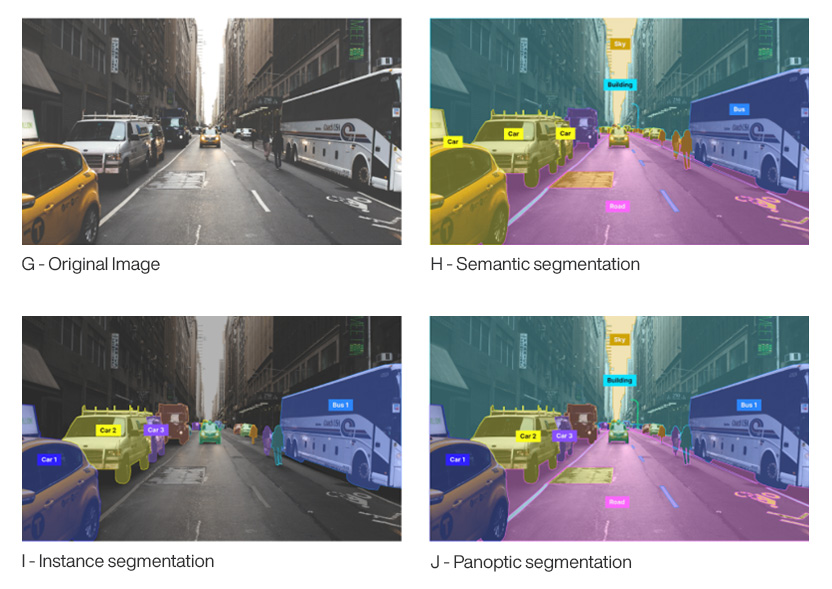
\includegraphics[width=12cm]{images/ss.jpg}
    	\caption{Semantic and Instance segmentation example. Courtesy of \cite{55_WinNT}}
    	\label{fig:SS}
    \end{figure}
    
    \subsection{Classical Semantic Segmentation}
    
    Most commonly used traditional segmentation techniques are threshold based technique \cite{56_otsu1979threshold}, histogram-based bundling, region-growing \cite{57_otsu1979threshold}, k-means clustering, watersheds, active contours, graph cuts, conditional and Markov random fields \cite{58_boykov2001fast}, sparsity based methods \cite{59_starck2005image}. However, in the recent years deep learning (DL) yielded a new generation of image segmentation models with state of the art performance. 
    
    \subsection{Deep Learning based  Semantic Segmentation}
    
    Deep learning based segmentation network can be classified into following categories \cite{60_minaee2021image}
    
    \begin{itemize}
    	\item Fully convolutional networks
    	\item Convolutional models with graphical models
    	\item Encoder-decoder based models
    	\item Multi-scale and pyramid network based models
    	\item R-CNN based models (for instance segmentation)
    	\item Dilated convolutional models and DeepLab family
    	\item Recurrent neural network based models
    	\item Attention-based models
    	\item Generative models and adversarial training
    	\item Convolutional models with active contour models
    \end{itemize}
    
    Deep learning based computer vision model most commonly use the convolutional neural network \cite{61_chen2017rethinking}, recurrent neural network (RNNs), and Long short term memory (LSTM), encoder-decoder \cite{62_badrinarayanan2017segnet} and generative adversarial networks (GANs) based networks \cite{60_minaee2021image}. The master thesis work is concentrated on the encoder-decoder based deep learning models. Encoder-Decoder based network are a two stage network that learns to map from input point to the output point. In the encoder stage the input data is compressed into a latent space representation $ z = f(x)$ and decoder decompress the latent space representation to the output $ a = g(z)$ \cite{63_goodfellow2014generative}. Latent representation of the input data in compressed form. It can be commonly observed in image-to-image translation problem as well as in sequence-to-sequence models in NLP. A reconstruction loss $ L(y, \hat{y})$ is defined at the output that measure the differences between the ground truth output $y$ and corresponding reconstruction $\hat{y}$. Autoencoders are the special version of the encoder-decoder models that have similar input and output.
    
    \begin{figure}[h]
    	\centering
    	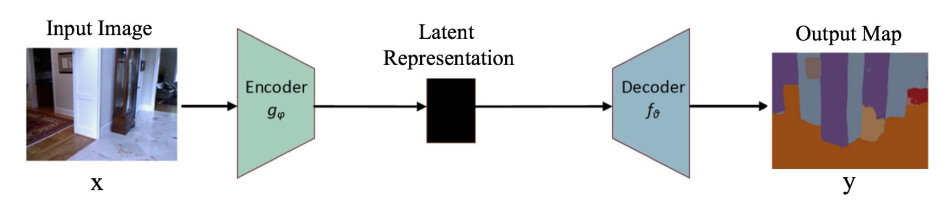
\includegraphics[width=14cm]{images/en_de.png}
    	\caption{Simple encoder-decoder architecture. Courtesy of \cite{60_minaee2021image}}
    	\label{fig:en_de}
    \end{figure} 		
    
    Most of the segmentation network are encoder-decoder based architecture. A novel semantic segmentation network was proposed by Noh et al \cite{64_noh2015learning}. The network is based on the deconvolution. The encoder network is based on the VGG 16-layer network and the decoder network takes the latent space encoding and outputs the pixel wise class probabilities. The segmentation mask and pixel-wise class labels are predicted by the deconvolutional and unpooling layers. The network generated a accuracy of 72.5 \% on the PASCAL VOC 2012 dataset. 
    
    \begin{figure}[h]
    	\centering
    	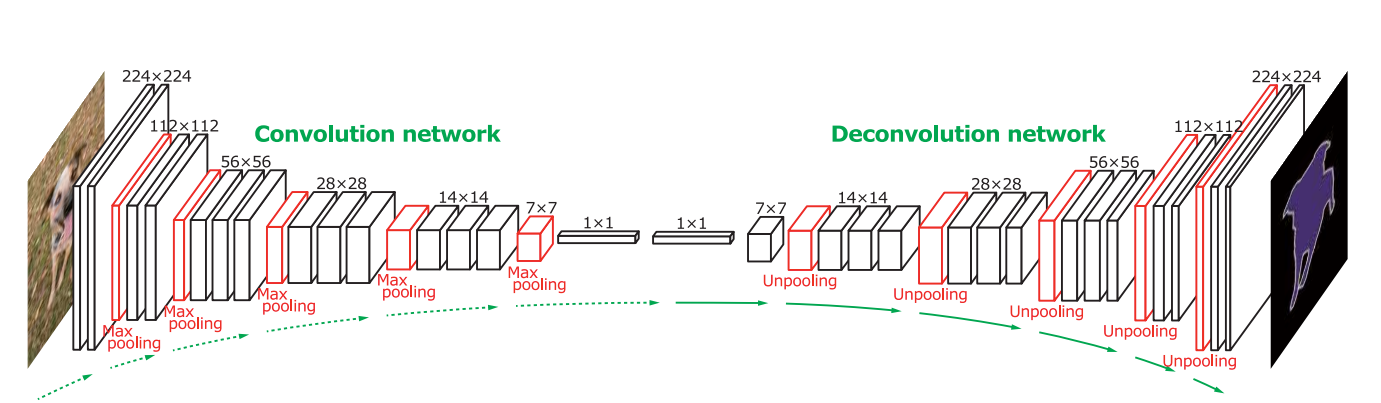
\includegraphics[width=14cm]{images/general_seg.png}
    	\caption{Simple encoder-decoder architecture. Courtesy of \cite{64_noh2015learning}}
    	\label{fig:general_seg}
    \end{figure} 
    
    Badrinarayanan et al proposed a convolutional encoder-decoder architecture for image segmentation called as SegNet \cite{62_badrinarayanan2017segnet}. The architecture of the SegNet described in the Figure \ref{fig:segnet}  
    
    \begin{figure}[h]
    	\centering
    	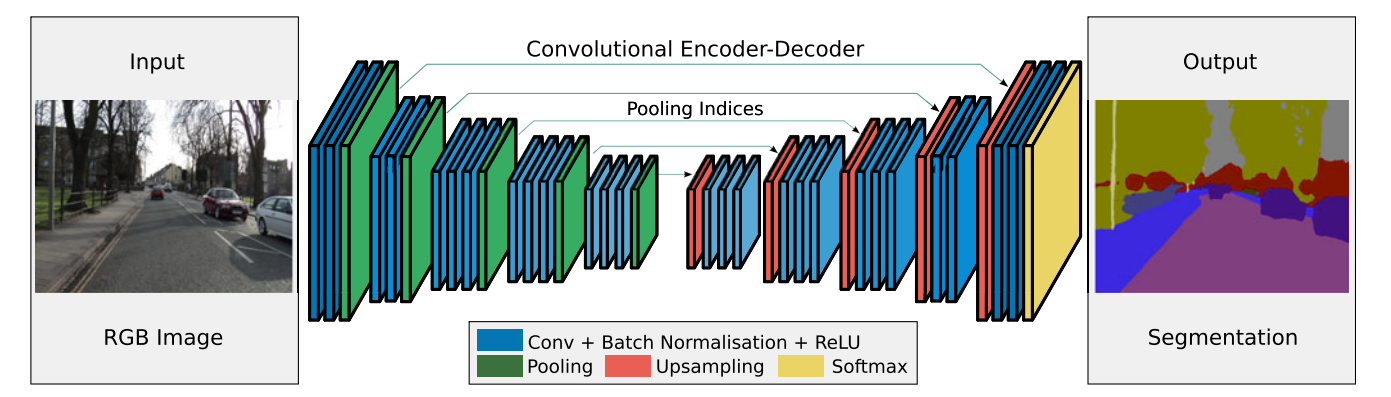
\includegraphics[width=14cm]{images/segnet.png}
    	\caption{SegNet architecture. Courtesy of \cite{62_badrinarayanan2017segnet}}
    	\label{fig:segnet}
    \end{figure} 
    
    The encoder part of the SegNet consist of 13 convolutional layers in the VGG16 network, and followed by the pixel wise classification layer. Decoder upsample the low resolution feature maps in a unique fashion. Non-linear upsampling is performed by using the pooling indices computed in the max-pooling step of the encoder. This process of reusing the encoder output helps to eliminate the need for learning to up-sample. Dense feature maps are generated by convolving with the trainable filters. To account for the uncertainty involved with the encoder-decoder network, scene segmentation is proposed \cite{65_kendall2015bayesian}. HRNet \cite{66_sun2019high} is the recently developed high resolution network by connecting the high to low resolution convolutions streams in parallel	and exchanging information between different resolutions. HRNet maintain high resolution representation through the encoding process. Many recent architecture use HRNet as the backbone. Other encoder decoder segmentation models are Stacked Deconvolutional Network \cite{67_fu2019stacked}, Linknet \cite{68_hu2018learning}, W-net \cite{69_xia2017w}.
    
    Many segmentation models are developed for medical application and among those U-Net \cite{70_ronneberger2015u} and V-Net \cite{71_milletari2016v} are the famous architecture. These architecture are now used outside of the medical domain.
    
    \begin{figure}[h]
    	\centering
    	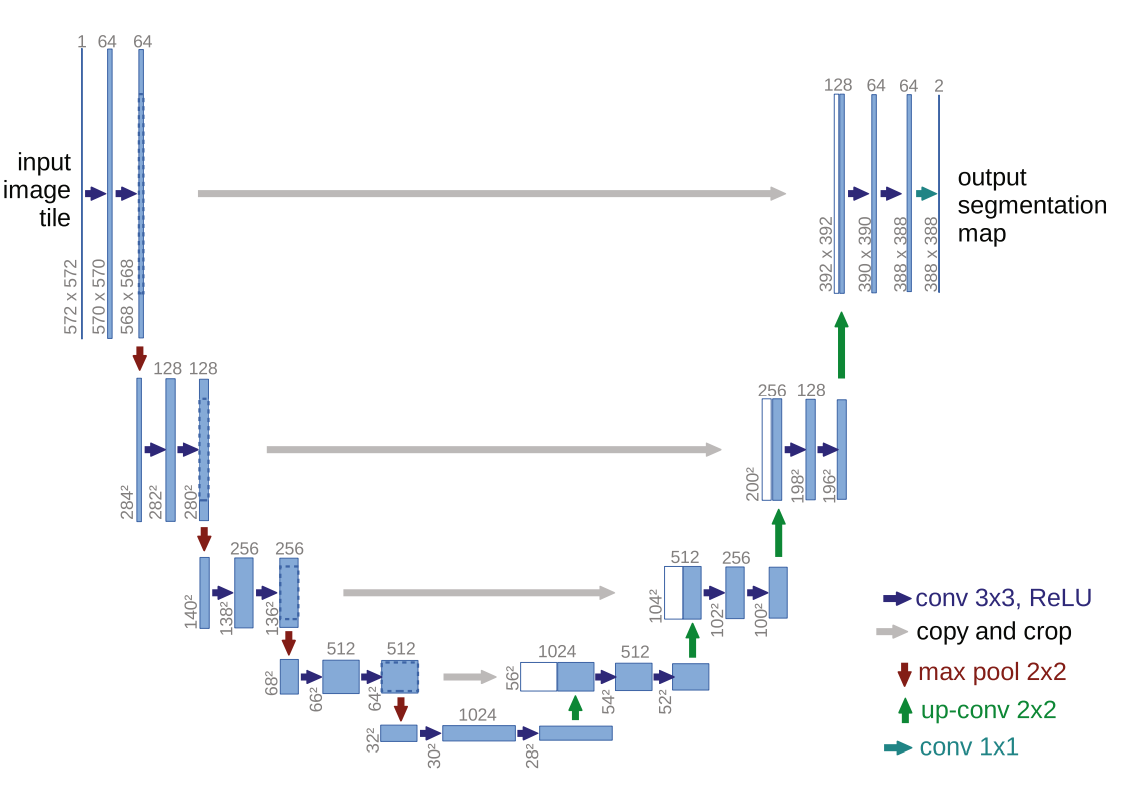
\includegraphics[width=14cm]{images/unet.png}
    	\caption{Unet architecture. Courtesy of \cite{70_ronneberger2015u}}
    	\label{fig:unet}
    \end{figure} 
	
	 Ronneberger et al \cite{70_ronneberger2015u} proposed a segmentation model to perform semantic segmentation on medical microscopy images. The architecture of the U-Net is described in Fig \ref{fig:unet}. The context is captured by the contracting part and localization of the target area is identified by the expanding decoder path. The network heavily dependent on the annotated images efficiently. The encoder part has a 3x3 convolutions features extractor, similar to the FCN-like architecture. The decoder part increases the dimensions and reducing the number of feature maps. The feature map from the encoder is mapped to the upscaled decoder to retain the pattern information. A 1x1 convolution at the output process the feature maps to generate segmentation output by categorizing each pixels of the input image to a particular class. Original U-Net was trained on the electronic microscopic images and outperformed by a large margin on the ISBI challenge. The network is fast and produce result on 512x512 image in less than a second on the modern GPU \cite{70_ronneberger2015u}, \cite{60_minaee2021image}. In a sequence data the information from the previous frames can be utilized to segment the current frame with a aim of improved performance in comparison to the segmentation without the temporal fusion. 
	 
    \section{Temporal Fusion in Semantic Segmentation}
    
    Semantic segmentation of sequence data aims to assign pixel-wise semantic labels to the video frames. It is a important task in the visual understanding \cite{72_jin2017video}. Strong representation of the feature map are important for the segmentation task. One of the common approach in the video segmentation is to perform the image segmentation to each frame independently. However the temporal information of the dynamic scenes are not captured by this approach. A common solution to the problem is to apply semantic segmentation to the each and every frame and add additional layer on top to capture the temporal data to extract the better features \cite{73_gadde2017semantic}, \cite{74_jin2017video}, \cite{75_nilsson2018semantic}. However, such approach doesn't help to improve the performance as feature needs to be computed at each and every frame. So a good approach is to apply the segmentation at key frames and reuse the already computed features for the other frames \cite{76_jain2019accel}, \cite{77_mahasseni2017budget}. A new highly efficient and low accuracy neural network based model is developed for semantic video segmentation called as Temporally Distributed Network (TDNet) \cite{78_hu2020temporally}. In TDNet feature extraction is distributed evenly across the sequential frames to eliminate the re-computation and then these features are combined together using the Attention Propagation Module (APM) to get the strong features for accurate segmentation \cite{78_hu2020temporally}. The pictorial representation of the same is described in the Fig \ref{fig:TDNet}. 
    
    \begin{figure}[h]
    	\centering
    	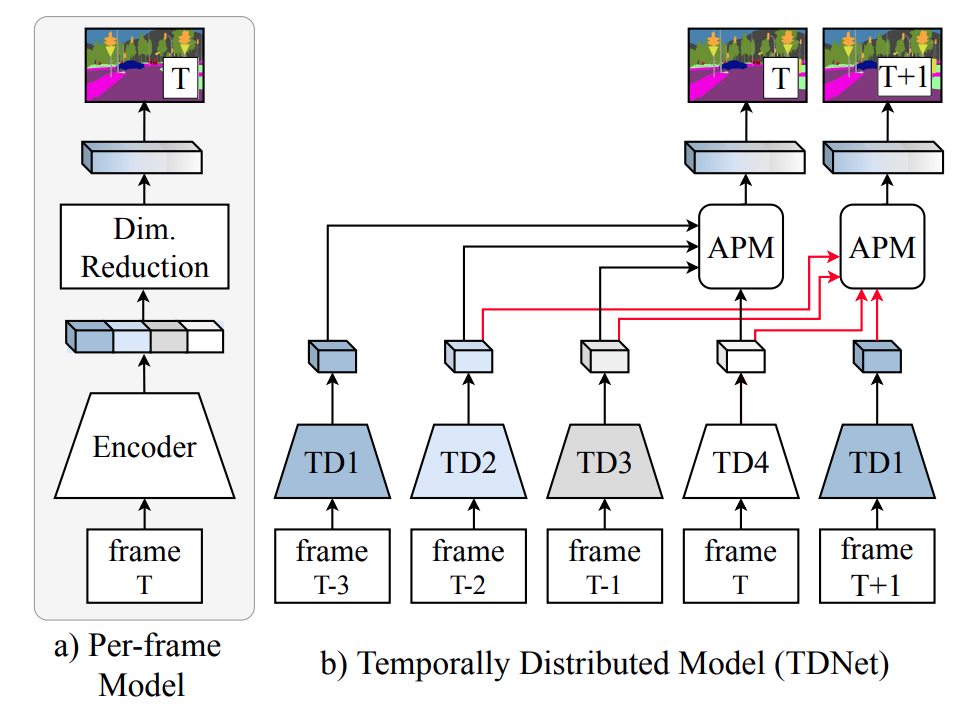
\includegraphics[width=12cm]{images/TDNet.png}
    	\caption{TDNet. Courtesy of \cite{78_hu2020temporally}}
    	\label{fig:TDNet}
    \end{figure}  
    
    \section{Limitations of Previous Work}
    
    The perception system of the modern ADAS uses segmentation to understand the surrounding environment by capturing the surrounding environment with the help of modern cameras. The high FPS data collected by the camera are in continuous sequence where the every frame is related to its previous frames. In general setting segmentation is performed on these frames to understand the object and their boundaries, number of objects, types of objects present in the frame. A work by Hou et al \cite{52_hou2019multi} integrate the camera pose data onto the computation of the depth maps, however similar strategy is not studied for a segmentation task. Also study of temporal data fusion in the latent space using LSTM is not studied in any of the previous work. This thesis aims to study the impact of temporal pose data onto the computation of the semantic segmentation and taking the previous frame data onto the current frame semantic segmentation task using LSTM network is studied. 
    
\end{document}
